\documentclass[10pt,twocolumn]{article}

% ---------------------------------------------------------------------------
% verl-apertus technical report
% ---------------------------------------------------------------------------
\usepackage[margin=1in]{geometry}
\usepackage[T1]{fontenc}
\usepackage{lmodern}
\usepackage{microtype}
\usepackage{amsmath}
\usepackage{amssymb}
\usepackage{booktabs}
\usepackage{graphicx}
\usepackage{subcaption}
\usepackage{xcolor}
\usepackage{enumitem}
\usepackage{authblk}
\renewcommand\Authsep{\qquad}
\renewcommand\Authand{\qquad}
\renewcommand\Authands{\qquad}
\setlength{\affilsep}{0.5em}
\usepackage[hidelinks]{hyperref}
\usepackage{titlesec}
\usepackage{dblfloatfix}
\setcounter{dbltopnumber}{2}
\renewcommand{\dbltopfraction}{0.9}
\renewcommand{\dblfloatpagefraction}{0.6}
\renewcommand{\topfraction}{0.9}
\renewcommand{\textfraction}{0.07}
\titlespacing*{\section}{0pt}{0.4ex plus 0.1ex}{0.2ex}

\setlength{\parskip}{0.15em}
\setlength{\parindent}{0pt}

\newcommand{\code}[1]{\texttt{\small #1}}

\title{\textbf{Enhancing Apertus Multimodal Perception via Tool-Use Reinforcement Learning}}
\author[1]{Mukhammadali Sayfiddinov}
\author[1]{Jovana Videnovic}
\affil[1]{Swiss AI Initiative, ETH Z\"urich}
\date{June 2026}

\begin{document}
\maketitle

\begin{abstract}
We bring a training recipe for visual reasoning with tools to Apertus. On this substrate we implement and train
(SFT$\rightarrow$GRPO) two capabilities: \\
(i) a \textbf{Grounding-box} capability trained by rewarding both the correct answer to an image-based question and the IoU of the grounding box. \\
(ii) a \textbf{Zoom-in} tool that, given a downsampled input image, re-encodes a crop of the \emph{original} full-resolution image to recover genuine detail; we initialize it from the grounding checkpoint so that it zooms the right region. As a control, we show that a \emph{no-magnification} crop tool is
inert: replacing cropped regions with random tokens does not change accuracy. \\
Both tools show performance gains on the validation set and on related benchmarks.
The core observations are that Apertus is able to improve its visual grounding, and that using this grounding to initialize the zoom-in policy lets zoomed-in crops help Apertus retrieve relevant details while minimizing the number of tokens needed to encode an input image.
\end{abstract}


\section*{Background: Apertus as a discrete-token VLM}
\label{sec:bg}

Apertus has no built-in vision transformer. Images enter through a single encoding path:
an aspect-preserving resize snaps an image's height and width to multiples of the
token block size (one token $=$ one $16\!\times\!16$ pixel block); the resized image is normalised and passed to a
discrete image tokenizer, Emu 3.5, and the resulting integer grid is rendered into an inline
string of visual-token markers that the LLM reads directly
as text. This differs from typical open-source models, e.g. the Qwen family, and hence a training recipe for Apertus is not readily available. Thus, we fill this gap by building a pipeline for vision-based SFT and RL training and then use it for two downstream tools: grounding-box and zoom-in.

% ---------------------------------------------------------------------------
% Grounding results -- full-width float anchored before the section so [t]
% resolves to the top of the grounding page rather than being deferred to the
% end of the document.
% ---------------------------------------------------------------------------
\begin{table*}[t]
\centering\small
\begin{tabular}{lcccl}
\toprule
& \multicolumn{3}{c}{VCoT test} & RefCOCO+ \\
\cmidrule(lr){2-4}\cmidrule(lr){5-5}
Model & Answer & Ground.\,Acc@0.5 & mIoU & Acc@0.5 \\
\midrule
base & 0.322 & 0.001 & 0.01 & 0.001 \\
SFT  & 0.434 & 0.185 & 0.21 & 0.274 \\
RL   & \textbf{0.497} & \textbf{0.313} & \textbf{0.295} & \textbf{0.309} \\
\bottomrule
\end{tabular}
\caption{Grounding. RL improves \emph{both} answer ($+13$\,pt over SFT, beats
base) and grounding ($+13$\,pt Acc@0.5).}
\label{tab:ground}
\end{table*}

\section*{Grounding-Box}
\label{sec:ground}
\paragraph{Tool.} The grounding tool exposes a single \code{bbox\_2d=[x1,y1,x2,y2]}
argument. The model gets no
rendered image back, and only the coordinates it emits are later scored with IoU,
alongside a separate final-answer call. Grounding is therefore an explicit output
capability.

\paragraph{Training.} SFT training traces come from a modified Visual-CoT dataset, with the reasoning traces kept and each
assistant turn ending by first drawing a box and then answering. The RL split is
built over the remaining single-word-answer rows. The reward scores the answer and localisation jointly:
\[
r = \underbrace{0.1}_{\text{disp}} + \underbrace{0.1}_{\text{bbox}} + 0.4\,\mathbb{1}[\text{ans}] + 0.4\,\mathrm{IoU}(\hat b, b^{\star}).
\]
Again, the model had to be rewarded for calling the tool correctly to avoid malformed tool calls.

\paragraph{Results.} We report two metrics separately: Answer is the
exact-match accuracy of the model's final answer, and Acc@0.5 is the
fraction of predicted boxes whose IoU with the gold box is $\ge\!0.5$ (mIoU
is the mean IoU over examples). The base model is scored format-agnostically from
its free text, since it does not emit the tool protocol.

Two points (Table~\ref{tab:ground}): (1)~the base model barely grounds
(Acc@0.5 $\approx$ 0, mIoU $0.01$), not for lack of spatial sense but because the checkpoint
almost never emits a usable box: most responses contain no tool call at all, and
the few boxes it does produce are placeholder templates or coordinates in an
unexpected format. (2)~SFT teaches the box-drawing protocol and RL sharpens it.
Because the answer$+$IoU reward is dense and correctness-aligned, GRPO improves
\emph{both} the answer (0.497, above base and SFT) and the localisation
(Acc@0.5 $0.185\!\to\!0.313$, mIoU $0.21\!\to\!0.30$), and the gain generalizes to a different RefCOCO+ referring-expression probe (Acc@0.5 $0.309$). This grounding-improved checkpoint is what we use to initialize the zoom-in policy next.

\section*{Zoom-in}
\label{sec:zoom}

\paragraph{Tool.} The zoom-in pipeline defines a verl-native tool exposing a single argument
\code{bbox\_2d = [x1,y1,x2,y2]} (description: ``Zoom in on a region for a
closer look at small details at available resolution''). Unlike verl's stock zoom
tool, which returns a PIL image, this returns the crop as a discrete-token
string. The crucial detail is what gets
cropped: the model's box is given in displayed-input space, sanitised back
to original pixels (rescaled and clamped to the image bounds), and the crop is taken from the \emph{original} full-resolution
image and re-encoded. Because of this, a small
region that occupied a handful of tokens in the input image now gets \emph{resolution gain}.

\paragraph{Training.} Both the SFT and RL datasets come from the CoF dataset. Crucially, rather than starting from the base image-SFT model, we initialize the zoom-in SFT from the grounding checkpoint above, so the policy already knows how to localise the region it should zoom into. SFT teaches the multi-turn protocol (Fig.~\ref{fig:zoom}):
each trace starts from the question and input image, has the assistant
\emph{think} and call the zoom tool, receives the crop back as a fresh token
string, and ends with a single answer call; traces use at most two crops. GRPO then optimises the same protocol on the sglang agent loop
against a simple reward,
\[
r=\min\!\big(1,\;\underbrace{0.1}_{\text{disp}}+\underbrace{0.1}_{\text{zoom}}
+0.9\,\mathbb{1}[\text{ans}]\big).
\]
The model had to be rewarded for correctly calling the display and zoom-in tools, as Apertus could not produce well-formatted tool calls even after SFT.
Two practical constraints shaped the runs. Long multi-turn rollouts are
memory-hungry, so the turn budget and KV-cache fraction have to be kept tight, and
the prompt/response split must leave enough room that a multi-turn zoom is never
truncated mid-trace. For experimentation, an image-token budget of 256 tokens (a 256$\times$256 pixel area) was used for both the input image and the returned, higher-resolution crops.

% ---------------------------------------------------------------------------
% Qualitative examples -- full-width float anchored early so [t] resolves to the
% top of the page (dblfloatfix prevents the usual figure* deferral to doc end).
% ---------------------------------------------------------------------------
\begin{figure*}[t]
\centering
\begin{subfigure}[t]{0.49\textwidth}
  \centering
  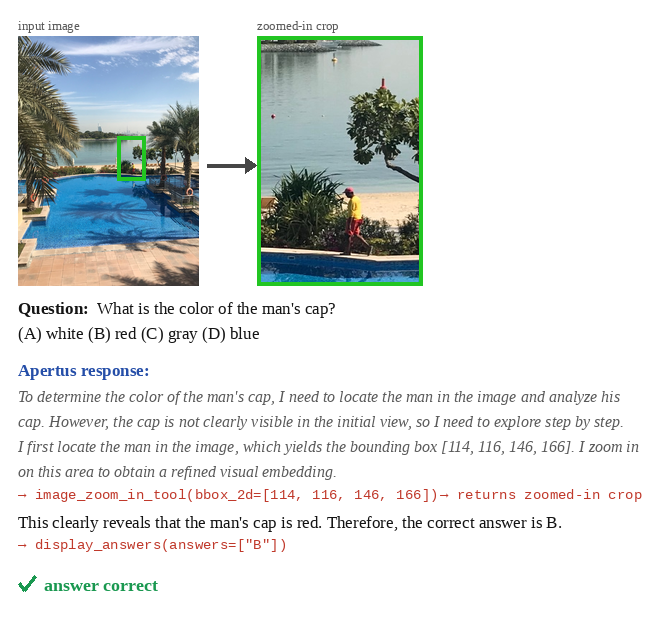
\includegraphics[width=\linewidth]{zoom_in.png}
  \caption{Zoom-in trace on V* Bench. The policy localises the target, calls the
  zoom tool on the \emph{original} image.}
  \label{fig:zoom}
\end{subfigure}\hfill
\begin{subfigure}[t]{0.49\textwidth}
  \centering
  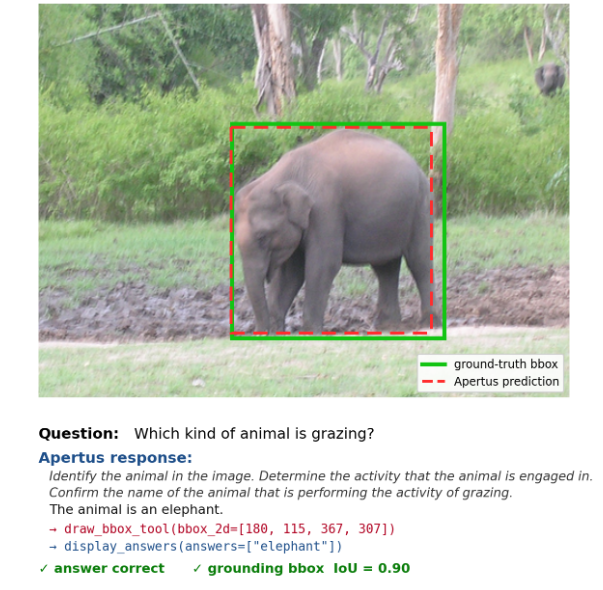
\includegraphics[width=\linewidth]{grounding_box.png}
  \caption{Grounding-box on VCoT. The policy emits a box (red) scored by IoU
  against the gold box (green), jointly with the answer.}
  \label{fig:ground}
\end{subfigure}
\caption{Qualitative examples. \emph{Left:} zoom as an \textbf{input} capability
(the crop feeds back into perception, adding resolution). \emph{Right:} grounding
as an \textbf{output} capability (the box is itself the deliverable).}
\label{fig:examples}
\end{figure*}

\paragraph{Results}

\begin{table}[t]
\centering\small
\begin{tabular}{lcc}
\toprule
Model & CoF eval  & V*Bench  \\
\midrule
base & 35.0          & 33.0 \\
SFT  & 54.4          & 45.2 \\
RL   & \textbf{64.9} & \textbf{49.3} \\
\bottomrule
\end{tabular}
\caption{Base, SFT and RL on the CoF evaluation set and
V*Bench, both at the 256-token budget. The SFT and RL zoom-in policies are
initialized from the grounding checkpoint. All numbers come from the sglang engine. The base model is scored from its free-text response, since it
never emits the tool protocol and a tool-gated metric would falsely read it near
zero.}
\label{tab:vstar}
\end{table}

Table~\ref{tab:vstar} shows that training now lifts \emph{both} the
CoF score ($35.0\!\to\!54.4\!\to\!64.9$) and V*Bench ($33.0\!\to\!45.2\!\to\!49.3$)
monotonically, even beating Apertus baseline with 2048 image token budget (40.1). This is the payoff of the grounding initialization: when we instead
trained zoom-in from the base image-SFT model, the same recipe left V*Bench flat and
RL even regressed it ($35.6\!\to\!32.5$), because the policy zoomed into the wrong
parts of the image; the grounding-initialized policy zooms the right region, so RL
no longer hurts V* and improves it. An ablation that withholds the tool confirms that zoom-in helps the model.

\paragraph{No-magnification control.} The gain above raises a question the
DeepEyes (Zheng et al. ICLR'26) recipe leaves open: does a crop tool help because it adds
\emph{resolution} (re-encoding a crop of the original full-resolution image) or
merely because it adds \emph{focus} (isolating a region the model has already
seen)? We answer it with a controlled no-magnification crop whose name and
schema are identical to those of the zoom tool, but which crops the already-perceived,
downscaled image and returns that sub-region at its native token count --- with
zero new pixels. This crop is inert: replacing its returned tokens with
random tokens of the same grid shape leaves accuracy unchanged (real =
noise), and once the multi-turn reasoning is trained in, removing the tool
entirely costs nothing RL simply discards it. A crop that adds no resolution
therefore carries no information, which disproves the focus interpretation: the
zoom tool's value is \textbf{resolution, not focus}.

\section*{Conclusion}
We built a vision SFT$\rightarrow$RL pipeline for Apertus, a discrete-token VLM, and
used it to add two visual tools. We first trained an explicit \textbf{grounding-box}
capability, and here RL is unambiguously beneficial: its dense answer$+$IoU reward
sharpens \emph{both} answering and localisation and transfers to RefCOCO+.

We then built \textbf{zoom-in} on top of the grounding checkpoint. The unifying
principle is that a visual input tool helps only when it supplies pixels the model
could not already see. Zoom-in does exactly this: re-encoding a crop of the
\emph{original} full-resolution image adds real resolution, and an ablation that
withholds the tool confirms the gain is causal. A no-magnification crop, which adds
focus but no new pixels, is by contrast inert (real = noise), refuting the implicit
DeepEyes premise that a crop tool's value is focus rather than resolution.

Initializing zoom-in from the grounding checkpoint closes the loop: a
base-initialized zoom policy zoomed the \emph{wrong} region and did not transfer to
V*Bench, where RL even regressed the score, whereas the grounding-initialized policy
lifts both CoF and V*Bench and reverses that regression. A model that grounds better
also zooms better, so tightening the grounding-to-zoom coupling is the natural next
step.
\end{document}
